\documentclass[english]{article}
\usepackage[T1]{fontenc}
\usepackage[utf8]{inputenc}
\usepackage[catalan]{babel}
\usepackage{lmodern}
\usepackage{microtype}
\usepackage{graphicx}
\usepackage{babel,blindtext}
\usepackage{geometry}
\usepackage{amsmath}
\usepackage{framed}
\usepackage{amsmath,amssymb,amsthm}
\usepackage{booktabs,colortbl,xcolor}
\usepackage{tabularx}
\usepackage[font=footnotesize,labelfont=bf]{caption}
 \geometry{
 a4paper,
 total={170mm,257mm},
 left=20mm,
 top=20mm,
 }

\begin{document}
\newcommand\makeAbstract{%
\begin{center}\textbf{Abstract (versió en català)}\end{center}
\begin{list}{}{\leftmargin=3em\rightmargin=\leftmargin}\item\relax
\small
L'anàlisi de dades d'expressió genètica és un dels grans reptes estadístics per a detectar expressions diferencials entre gens sota una condició donada. La idea principal d'aquest treball, és la creació d'un protocol d'anàlisi interactiu de matrius d'expressió genètica. Es presenten mètodes estadístics com l'anàlisi de la variància (ANOVA). Mètodes de correcció per multiplicitat de contrastos també queden descrits. S'utilitzen mètodes gràfics com els mapes de calor. Tot aquest protocol d'anàlisi s'implementa en una aplicació web desenvolupada amb Shiny.
\end{list}\par\vspace{6mm}%
\begin{center}\textbf{Abstract (versión en castellano)}\end{center}
\begin{list}{}{\leftmargin=3em\rightmargin=\leftmargin}\item\relax
\small
El análisis de datos de expresión genética es uno de los grandes retos estadísticos para detectar expresiones diferenciales entre genes mediante una condición establecida. La idea principal de este trabajo, es la creación de un protocolo de análisis interactivo de matrices de expresión genética. Se presentan métodos estadísticos como el análisis de la varianza (ANOVA). Métodos de corrección por multiplicidad de contrastes también quedan descritos. Se utilizan métodos gráficos como los mapas de calor. Todo este protocolo de análisis se implementa en una aplicación web desarrollada con Shiny.
\end{list}\par\vspace{6mm}%
\begin{center}\textbf{Abstract (English version)}\end{center}
\begin{list}{}{\leftmargin=3em\rightmargin=\leftmargin}\item\relax
\small
 Data gene expression analysis is one of the major statistical challenges to detect differential expressions between genes under a given condition. The main idea is the creation of an interactive analysis protocol of gene expression matrix. Methods are presented for detecting differential expression using statistical hypothesis testing methods including analysis of variance (ANOVA). Methods for multiple testing correction and their application are described. Graphical methods such as heatmaps are used. This analysis protocol is implemented in a web application developed in Shiny.
\end{list}\par\vspace{6mm}%
}

\title{
\textsc{Treball de final de grau}\\[2.6cm]
{\LARGE \bfseries Protocol d'anàlisi per a dades d'expressió gènica amb Shiny}\\{\Large\bfseries Grau d'Estadística Aplicada}\\[5cm]
}

\author{
\textsc{Autor:} Antonio Rodríguez Gómez
}

\date{
\textsc{Supervisor:} Mercè Farré \\[1em]
\today
}

\maketitle
%%% Local Variables:
%%% mode: latex
%%% TeX-master: "test"
%%% End:

\thispagestyle{empty}
\clearpage
\twocolumn[\makeAbstract]
\thispagestyle{empty}
\clearpage
\tableofcontents
\clearpage
\section{Introducció}
Un dels reptes més grans de la biologia actualment és analitzar els volums massius de dades creats, per exemple, en la seqüenciació de DNA. La gran evolució de les tècniques de recollida de dades biològiques ha fet que sigui necessari el desenvolupament de metodologies eficients a l'hora de tractar i analitzar les dades. La disciplina que recull aquestes metodologies s'anomena bioinformàtica.
\\

La bioinformàtica és un àrea emergent interdisciplinària que s'ocupa de l'aplicació de l'informàtica a la recopilació, emmagatzematge, organització, anàlisis, manipulació, presentació y distribució d'informació relativa a les dades biològiques o mèdiques.
\\

Aquest treball s'ha centrat en l'anàlisis de bases de dades d'expressió genètica a partir de diferents condicions experimentals. Al llarg del treball s'utilitzen técniques per analitzar aquests tipus de dissenys on l'objectiu recau en veure quins gens s'expressen significativament sota condicions experimentals establertes.
\\

Amb aquesta premissa, el treball també s'ha enfocat en crear un aplicatiu web capaç de fer un anàlisi estadístic de les matrius d'expressió gènica. L'aplicatiu ha sigut programat amb R, per mitjà del paquet Shiny. Aquest paquet és capa\c{c} d'implementar el codi R de manera interactiva. No només implementa el codi R, sinó també és capaç d'interactuar amb diferents llenguatges com html, css o java. Tot el conjunt de l'aplicació ha sigut organitzada i compartida per mitjà d'un repositori creat en la plataforma GitHub. D'aquesta manera el codi queda a disposició de qualsevol usuari que vulgui utilitzar-lo o consultar els métodes empleats.

\subsection{Introducció als conceptes bàsics de la bioinformàtica}
%(PDF de bioinformatica)(ttp://masteres.ugr.es/moea/pages/curso201314/tfm1314/tfm-septiembre1314/memoriamasterdanielparrasburgos/!)

Cada organisme es defineix pel seu material genètic, el genoma. La informació genètica la trobem emmagatzemada en una macromolècula anomenada DNA, que es troba al nucli de cada cèl·lula.
\\

Un gen consisteix en un segment de DNA que conté el codi per a la producció d'una proteïna. Una única cadena d'ADN conté milers de gens, cadascun sintetitza una proteïna concreta. Per fer-nos a la idea, els humans tenim al voltant de 20.000 gens. La longitud i seqüència d'un gen determina la grandària i la forma de la proteïna que sintetitza i quina funció tindrà aquesta proteïna dins de l'organisme.
\\

La dotació de gens que presenta una espècie, s'anomena genotip, i l'aparen\c{c}a externa d'un caràcter genètic, l'anomenem fenotip. L'expressió del genotip ve determinat, a més de per la càrrega genètica, per l'ambient i el comportament dels éssers vius. Si un gen no s'expressa en un individu, aquest tindrà el mateix fenotip que un individu que no presenti el gen. Però com podem arribar a obtenir una mesura de l'expressió dels gens? Existeixen tècniques per quantificar-ho? La resposta és sí.
\\

La mesura de l'expressió gènica generalment és dur a terme quantificant els nivells de producte del gen. Una tècnica molt utilitzada de mesura de l'expressió gènica que utilitza ARN missatger és la denominada transcripció inversa, seguida de la reacció en cadena quantitativa de la polimerasa (qPCR \footnote{Aquesta tècnica serveix per amplificar un fragment d'ADN i la seva utilitat rau en el fet que després de l'amplificació resulta molt més fàcil identificar material genètic amb una gran precisió.}). Una de les seves principals característiques és la seva sensibilitat, ja que només necessita una única molècula per iniciar el procés de replicació. A més, és molt robusta gràcies al fet que permet utilitzar diferents productes biològics, com cabells, teixits, mucoses, sang, etc. Aquesta tècnica és fonamental per l'anàlisi de dades d'expressió gènica, perquè per l'obtenció d'aquestes dades es requereix una quantitat suficientment gran de producte biològic que no sempre és de fàcil obtenció, per tant, és important disposar d'una tècnica que faciliti la seva replicació de forma controlada, robusta i eficient.
\\

Centres de genòmica s'encarreguen de fer aquests processos i de retornar els resultats en matrius de dades on es recullen els nivells d'expressió per a cada gen. Per tant, és important fer un bon disseny experimental ja que aquests procesos són costosos i requereixen de temps, a més del biaix estadístic que es pot generar.


\subsection{Cas d'estudi: Protocol d'análisi d'un OpenArray}
Des de la facultat de veterinaria de l'Universitat Autònoma s'han dut a terme estudis experimentals sobre l'expressió dels gens animals en certes condicions experimentals. L'aplicatiu web ha sigut creat per donar suport estadístic al grup d'investigació de la UAB \textbf{Nombre del grupo}.
\\

El cas d'estudi que el treball ha contemplat consisteix en un experiment amb animals, concretament, amb porcins. Durant l'experiment s'administraven diferents tractaments/dietes als porcins. D'aquesta manera es volia veure l'afectació d'alguns tractaments en la regulació intestinal i com afectava al creixement dels porcins.
\\

Les dades utilitzades en aquest treball han sigut proporcionades per \textbf{Nombre del grupo} per mitjà de la tecnologia OpenArray. El material biològic que s'ha utilitzat per l'obtenció de les dades, han sigut diferents tipus de teixits del intestí. Els gens van ser escollits amb criteris científics pels investigadors i tenen un significat concret dins del funcionament de la regulació intestinal.
\\

Encara que l'aplicatiu web s'ha creat a partir d'aquest estudi, la idea ha sigut generalitzar el codi per poder utilitzar-ho amb altres dissenys experimentals.

\section{Protocol d'anàlisi}
%https://stats.stackexchange.com/questions/78920/mathematical-explanations-behind-anova
En aquest apartat queden definits els mètodes estadístics utilitzats en el protocol d'anàlisi. Cada mètode ha sigut implementat en l'aplicatiu i més endavant es mostren els resultats del cas d'estudi.
\subsection{Anàlisi de la variància (ANOVA)}
L'anàlisi de la variància (ANOVA) és el mètode clàssic per comparar mitjanes entre grups dos grups o més.
\\

\textbf{Observació.} Hi ha una sèrie de supòsits que s'han de fer abans que s'apliqui l'ANOVA, la desviació en aquests supòsits portaran a resultats que poden ser enganyosos o inexactes. Aquests supòsits inclouen la independència, normalitat i variància constant dels errors. En algunes situacions, hi ha transformacions que poden ser utilitzades per evitar les violacions d'aquests supòsits, com ara la transformació logarítmica de les dades.
\\

Suposem que tenim $N$ observacions repartides en $k$ grups i definim $n=\frac{N}{k}$. Llavors $x_{ij}$ seria l'individu $j$ corresponent al grup $i$. En aquest cas assumim que l'estudi és balancejat, és a dir, el nombre d'individus per grup és el mateix. Denotem $\bar{x.}$ com la mitjana de la mostra global, i $\bar{x_{i}}$ com la mitjana del grup $i$.
Les observacions es poden tornar a escriure com:
\begin{equation*}
x_{ij} = \bar{x.} + (\bar{x_{i}} - \bar{x.}) + (x_{ij} - \bar{x_{i}})
\end{equation*}
Això ens porta al següent model:
\begin{equation*}
x_{ij} = \mu + \alpha_{i} + \epsilon_{ij}
\end{equation*}
on $\mu$ i $\alpha_{i}$ són la mitjana global i la mitjana del grup $i$ respectivament. S'assumeix que el terme d'error $\epsilon_{ij}$ és iid i segueix una distribució normal
\begin{equation*}
\epsilon_{ij} \sim \mathcal{N}(\mu,\,\sigma^{2})\,
\end{equation*}
La hipòtesi nul·la en un model ANOVA és que les mitjanes dels grups són iguals, és a dir:
\begin{equation*}
\alpha_1 = \alpha_2 = ... = \alpha_k
\end{equation*}
Si això és cert, el terme d'error per a la diferència de grups queda definit com:
\begin{equation*}
\bar{x_{i}} - \mu \sim \mathcal{N}(0,\,\frac{\sigma^{2}}{n}=\bar{\sigma}^2)\,
\end{equation*}
Es pot mesurar la quantitat total de variabilitat entre observacions sumant els quadrats de les diferències entre cadascun $\bar{x}.$ i $x_{ij}$:

\begin{equation*}
SST(\text{Suma de quadrats totals}) = \sum_{i=1}^{k} \sum_{j=1}^{n_{i}} (x_{ij} - \bar{x}.)^2
\end{equation*}
La variabilitat total es pot desglossar en 2 termes:
\begin{enumerate}
\item La variabilitat entre grups:
\begin{equation*}
SSG = \sum_{i=1}^{k} n_{i}(\bar{x}_{i} - \bar{x}.)^2
\end{equation*}
amb $k-1$ graus de llibertat.
\item La variabilitat intra grups:
\begin{equation*}
SSE = \sum_{i=1}^{k} \sum_{j=1}^{n_{i}} (x_{ij} - \bar{x_{i}})^2
\end{equation*}
amb $N-k$ graus de llibertat.
\end{enumerate}
Per tant, podem escriure la suma de quadrats totals com:
\begin{equation*}
SST = SSG + SSE
\end{equation*}

Si la variabilitat entre grups és gran en relació amb la variabilitat intra grups, llavors les dades suggereixen que les mitjanes de les poblacions són significativament diferents. Si no existeixen diferencies, entre els grups, esperaríem que les mitjanes quadràtiques
\begin{equation*}
MSG = \frac{SSG}{(k-1)}
\end{equation*}
\begin{equation*}
MSE = \frac{SSE}{(N-k)}
\end{equation*}
siguin similars. El test estadístic ANOVA es defineix com la ràtio entre les dues mitjanes quadràtiques:
\begin{equation*}
F = \frac{MSG}{MSE}
\end{equation*}
L'estadístic $F$ segueix una distribució F de Snedecor amb $k-1$ i $N-k$ graus de llibertat. Si la hipòtesi nul·la és certa, $F$ seria proper a 1. D'altra banda, si la mitjana quadràtica entre grups $MSG$ és gran, suposaria un valor gran de l'estadístic F. Bàsicament, l'ANOVA examina les dues fons de la variància total i mira quina part contribueix més. Per aquest motiu, s'anomena anàlisi de la variància encara que la intenció sigui comparar les mitjanes dels grups.
\\

\subsubsection{Anova per a dissenys desbalancejats}
En procés...
\clearpage

\subsection{Correcció per multiplicitat de contrastos}
%http://www.stat.cmu.edu/~genovese/talks/hannover1-04.pdf
%Limma
Un problema comú què ens podem trobar a qualsevol investigació és voler comparar més de 2 grups de dades per detectar possibles diferències entre ells. La utilització de models d'ANOVA ens pot permetre detectar diferències, a escala global, entre les mitjanes involucrades, però en moltes ocasions volem detectar les diferències entre grups concrets. Aquest cas només és possible mitjançant l'ús dels Procediments de Comparacions múltiples (PCM).
\\

En aquest treball el nostre interès no és avaluar si un o dos gens concrets s'expressen d'una forma diferencial entre les condicions considerades. Volem veure això a un nivell global i respondre a una pregunta com: Quins gens s'expressen d'una manera diferent (diferencial si utilitzem la literatura biològica) en els grups/tractaments que considerem? L'objectiu és poder contestar aquesta pregunta de manera que puguem controlar les vegades que afirmem expressions diferencials quan realment no la tenen (Error de tipus I).
\\

Si numerem els gens $i = 1,...,N$ llavors per a l'i-èssim gen estem considerant el següent contrast:
\begin{itemize}
\item $H_{0}$ : El gen i no té una expressió diferencial entre les condicions considerades.
\item $H_{1}$: El gen i té una expressió diferencial entre les condicions considerades.
\end{itemize}
Si plantegem aquest contrast per a cada gen, podem denotar com $G={1,..,N}$ el conjunt d'hipòtesis nul·les que estem avaluant. El número d'hipòtesis que avaluem és conegut a priori, ja que correspon al número de gens que volem avaluar. És important destacar que en els estudis d'investigació en intentar acceptar o rebutjar la hipòtesi nul·la ($H_{0}$) es poden cometre dos tipus d'errors:
\begin{itemize}
\item Error de tipus I: Rebutjar $H_{0}$ quan realment és certa.
\item Error de tipus II: No rebutjar $H_{0}$ quan realment és falsa.
\end{itemize}
Imaginem que fem un test contrastant diferencies entre mitjanes, i fixem un nivell de significació $\alpha=0.05$, i sabem que la hipòtesis nul·la és certa; llavors l'error de tipus I serà exactament el nivell de significació $\alpha$. Per tant, podem definir la probabilitat de tenir un fals positiu en un test, és a dir, rebutjar $H_{0}$ quan realment és certa:
\begin{equation*}
P(\text{Fals positiu}) = \alpha
\end{equation*}
\begin{equation*}
P(\text{No cometre l'error}) = 1 - \alpha
\end{equation*}
Per tant, si definim $m$ tests d'hipòtesis podem definir la probabilitat d'almenys tenir 1 fals positiu com:
\begin{equation*}
P(\text{No cometre l'error en m tests}) = (1 - \alpha)^m
\end{equation*}
\begin{equation*}
P(\text{Almenys 1 fals positiu en m tests}) = 1 - (1 - \alpha)^m
\end{equation*}
Per exemple, si tenim 1 test, i fixem $\alpha=0.05$, la probabilitat d'obtenir almenys 1 fals positiu és de:
\begin{equation*}
P(\text{Almenys 1 fals positiu}) = 1-(1-0.05)= 0.05
\end{equation*}
Si ara tenim 50 tests i calculem la mateixa probabilitat:
\begin{equation*}
P(\text{Almenys 1 fals positiu}) = 1-(1-0.05)^{50}= 0.92
\end{equation*}

Aquí recau el gran problema de la multiplicitat de contrastos, podem observar que si fem un test moltes vegades, hi ha una inflació en l'error de tipus I.
\begin{center}
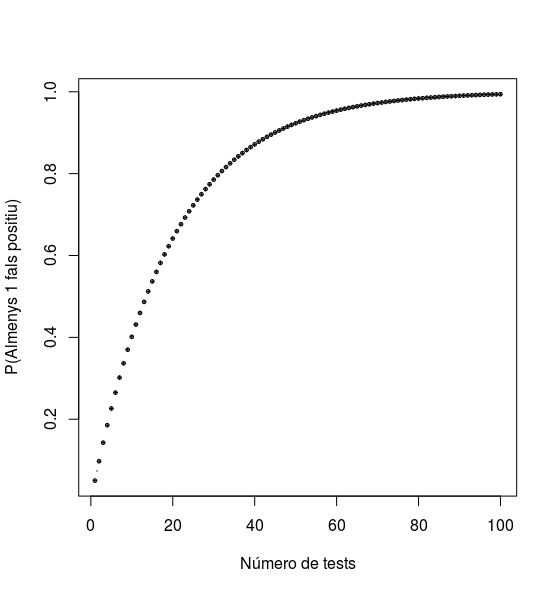
\includegraphics[scale=0.5]{FalsPositiu.png}
\captionof{figure}{Gràfic contraposant el nombre de tests amb la probabilitat d'obtenir almenys 1 fals positiu. S'observa un increment en la probabilitat quan augmenta el nombre de tests.}
\end{center}
En el nostre estudi es important tenir clar aquest problema, ja que si tenim molts gens, i no apliquem una correcció, podem caure en l'error d'afirmar que un gen s'expressa diferencialment quan realment no ho fa.
\subsubsection{False discovery Rate}
%http://www.gs.washington.edu/academics/courses/akey/56008/lecture/lecture10.pdf
%https://rpubs.com/Joaquin_AR/236898
Existeixen molts mètodes per corregir el problema de la multiplicitat de contrastos. El més simple és el mètode de Bonferroni, on cada p valor es multiplica pel nombre de tests realitzats (acotant la probabilitat màxima a 1). És un mètode molt conservador i no és el més indicat per al nostre cas d'estudi.
Per a escenaris de large-scale multiple testing com els estudis de genòmica, els quals es realitzen milers de test de forma simultània, el resultat d'aquests mètodes és massa conservador i impedeix que es detectin diferències reals. Una alternativa és controlar el false discovery rate.
\\

El false discovery rate ($FDR$) es defineix com la proporció esperada de falsos positius d'entre tots els tests considerats com significatius. L'objectiu de controlar el false discovery rate es establir un límit de significació per a un conjunt de tests tal que, d'entre tots els tests considerats com significatius, la proporció d'hipòtesis nul·les (falsos positius) no superin un determinat valor.
Un altre avantatge afegit és la seva fàcil interpretació, per exemple, si un estudi publica resultats estadísticament significatius per a un $FDR$ del 10$\%$, el lector té la seguretat que, com a màxim, un 10$\%$ dels resultats considerats com a significatius són realment falsos positius.
\\
La primera aproximació per controlar el FDR va ser descrita per Benjamini $\%$ Hochberg en 1995. D'acord amb la seva publicació si es desitja controlar que en un estudi amb $n$ comparacions el $FDR$ no superi un percentatge $d$ hem de:

\begin{itemize}
\item Ordenar els $n$ tests de menor a major $pvalor$ ($p_{1}$,$p_{2}$,... $p_n$).
\item Es defineix $k$ com l'última posició per la qual es compleix que $p_i \leq d\frac{i}{n}$.
\item Es consideren significatius tots els $pvalors$ fins a la posició $k$ ($p_{1}$,$p_{2}$,... $p_k$).

\end{itemize}

El mètode proposat per Benjamini $\&$ Hochberg assumeix a l'hora d'estimar el nombre d'hipòtesis nul·les erròniament considerades falses, que totes les hipòtesis nul·les són certes. Com a conseqüència, l'estimació del $FDR$ està inflada i és un mètode conservador. Per poder veure l'afectació d'utilitzar un mètode com Bonferroni o utilitzar el métode Benjamini $\&$ Hochberg, tenim la següent taula d'exemple:
\\
\begin{table}[ht]
\centering
\begin{tabular}{rrrr}
\hline
& Pvalor & Bonferroni & Benjamini$\&$Hochberg \\
\hline
1 & 0.0010 & 0.0550 & 0.0037 \\
2 & 0.0020 & 0.11 & 0.0069 \\
3 & 1 & 1 & 1 \\
4 & 0.0010 & 0.0550 & 0.0037 \\
5 & 0.0010 & 0.0550 & 0.0037 \\
6 & 0.0010 & 0.0550 & 0.0037 \\
7 & 0.25 & 1 & 0.3929 \\
8 & 0.48 & 1 & 0.6286 \\
9 & 0.09 & 1 & 0.1650 \\
10 & 0.51 & 1 & 0.6523 \\
\hline
\end{tabular}
\caption{A l'exemple de la taula hi ha una columna amb les $pvalors$ sense corregir, un altre amb la correcció de Bonferroni i per últim una amb la correcció proposada per Benjamini$\&$Hochberg, per a un total de 55 $pvalors$ (Encara que només es mostren els 10 primers). Observem que Bonferroni és un mètode molt més conservador i cap $pvalor$ és significatiu. (Dels 55 $pvalors$, 0 són significatius amb Bonferroni). En canvi, amb el mètode de Benjamini$\&$Hochberg, observem que del total de $pvalors$, hi ha 26 significatius.(En aquest cas hem fixat un $\alpha=0.05$ i un $FDR=0.05$) }
\end{table}

A l'hora de decidir quin tipus de correcció aplicar, és important utilitzar un mètode adequat per tal d'obtenir resultats més acurats. En els estudis exploratoris és d'esperar que la proporció d'hipòtesis nul·les falses, és a dir, tests que són realment significatius, sigui alta. Per tant, mètodes que només depenen del nombre de tests no són els més potents per aquest tipus d'estudis, com hem vist anteriorment.

\subsection{Comparacions múltiples}
Un cop realitzat l'anàlisi de la variància i si aquest confirma l'existencia de diferències significatives entre els grups o tractaments, és convenient investigar quines mitjanes són diferents. El conjunt de tècniques que tracten aquest problema es denominen \textit{contrastos per comparacions múltiples}.
\\

\subsubsection{Métode de Tukey (\textit{Honestly-significant-difference})}
%http://www.ugr.es/~bioestad/guiaspss/practica7/ArchivosAdjuntos/ComparacionesMultiples.pdf
%http://www2.hawaii.edu/~taylor/z631/multcomp.pdf
Recordem que quan el nombre de possibles comparacions és elevat, per a un nivell de significació $\alpha$ donat, pot conduir a una inflació de l'error de tipus I, com també hem vist quan parlàvem de multiplicitat de contrastos.
\\
Per identificar quins tractaments són significativament diferents entre ells i corregir el problema de la inflació de l'error de tipus I, hem utilitzat el mètode de Tukey i les seves hipòtesis són:

\begin{equation*}
H_{0}: \mu_1 = \mu_2 = ... = \mu_k
\end{equation*}
\vspace{-0.5cm}
\begin{equation*}
H_{1}: \mu_1 \neq \mu_2 \neq ... \neq \mu_k
\end{equation*}
\\
Aquest contrast es basa en la distribució del rang estudentitzat, que es defineix a partir del nombre de grups a comparar i dels graus de llibertat de l'estimador de la variància. Aquests tipus de procediments, permeten superar les dificultats que hi ha quan augmentem el nombre de grups a comparar i no podem controlar els falsos positius. En general, són mètodes conservadors, es a dir, la probabilitat real de rebutjar la hipòtesi nul·la quan és certa és menor que el nivell de significació $\alpha$ fixat.
\\

Per definir el rang estudentitzat, suposem que disposem de $k$ observacions independents $y_1,y_2,...,y_k$ d'una distribució Normal amb mitjana $\mu$ i variància $\sigma^2$. Suposem també que disposem d'un estimador $S^2$ de $\sigma^2$ que té $v$ graus de lliberat i és independent de les $y_i$. Definim $R$ com el rang d'aquest conjunt d'observacions,
\begin{equation*}
R = max(y_i) - min(y_i)
\end{equation*}
Sota aquestes condicions, es defineix el rang estudentitzat com el quocient,
\begin{equation*}
\frac{max(y_i) - min(y_i)}{S} = \frac{R}{S}
\end{equation*}
que es denota com $q_{k,v}$. Aquest estadístic segueix una distribució que depèn dels paràmetres $k$ i $v$, coneguda com la distribució del rang estudentitzat. L'estadístic de contrast que utilitza el test de Tukey, també segueix una distribució del rang estudentitzat. L'estadístic compara les mitjanes dels grups $j$ i $k$, i ve donat per la següent equació:
\begin{equation*}
HSD = q_{I,N-I}(\alpha)\sqrt{\frac{\hat{S}^2}{n}} ,
\end{equation*}

\begin{equation*}
q_{I,N-I}(\alpha) = \frac{\bar{X}_j - \bar{X}_k}{\sqrt{\frac{\hat{S}^2}{n}}}
\end{equation*}
on $\hat{X}_j$ i $\hat{X}_k$ són la mitjana del grup $j$ i $k$, respectivament, i $\hat{X}_j > \hat{X}_k$. $\hat{S}^2$ és l'estimació de la variància del error o residual; i $n$ és la grandària mostral per a tots els grups; on $I$ i $N-I$ són els graus de llibertat de la distribució del rang estudentitzat ($I$ correspon al nombre de nivells que té el factor, $N$ correspon a la grandària mostral).En el cas de tenir grandàries mostrals diferents entre els nivells del factor, hem d'utilitzar un altre $n$ (mitjana harmònica):
\begin{equation*}
n_h = \frac{t}{\sum_{i=1}^{t}\frac{1}{n_i}}
\end{equation*}
\\

La diferència entre mitjanes serà significativa amb un nivell de significació $\alpha$ si
\begin{equation*}
|\bar{X}_j - \bar{X}_k |> HSD
\end{equation*}
L'interval de confian\c{c}a per a la diferència de mitjanes el definim com:
\begin{equation*}
IC(\mu_j - \mu_k)_{(1-\alpha)}= (\bar{X}_j - \bar{X}_k) \pm q_{I,N-I,1-\alpha}\sqrt{\frac{\hat{S}^2}{n}}
\end{equation*}
Si l'interval de la diferència inclou el 0, no rebutjem la hipòtesi nul·la del test i per tant, no hi ha diferències entre $\mu_j$ i $\mu_k$.
\subsection{Mètodes descriptius visuals}
%http://mural.uv.es/rata3/PECS/Genomica%20Funcional%20y%20Analisis%20de%20Microarrays%20PEC2.pdf
A l'hora de crear el protocol d'anàlisi teníem la necessitat de descriure el comportament de l'expressió dels gens segons unes covariables. Una manera de veure aquests patrons era amb l'ús de tècniques visuals, que tenen una base matemàtica que explicarem en els següents apartats.
\subsubsection{Heatmap}
%http://wpd.ugr.es/~bioestad/guia-spss/practica-8/#8
%http://www.opiniomics.org/you-probably-dont-understand-heatmaps/
Un \textit{Heatmap} (o mapa de calor) és una representació gràfica de dades on els valors individuals continguts en una matriu es representen com a colors.
\\

En mapes de calor, les dades es mostren en una quadrícula on cada fila representa un gen i cada columna representa una mostra. El color i la intensitat de les caselles s'utilitzen per representar canvis (no en valor absolut) de l'expressió gènica.
\\

Tenim el següent exemple que podem obtenir a l'aplicatiu:
\begin{center}
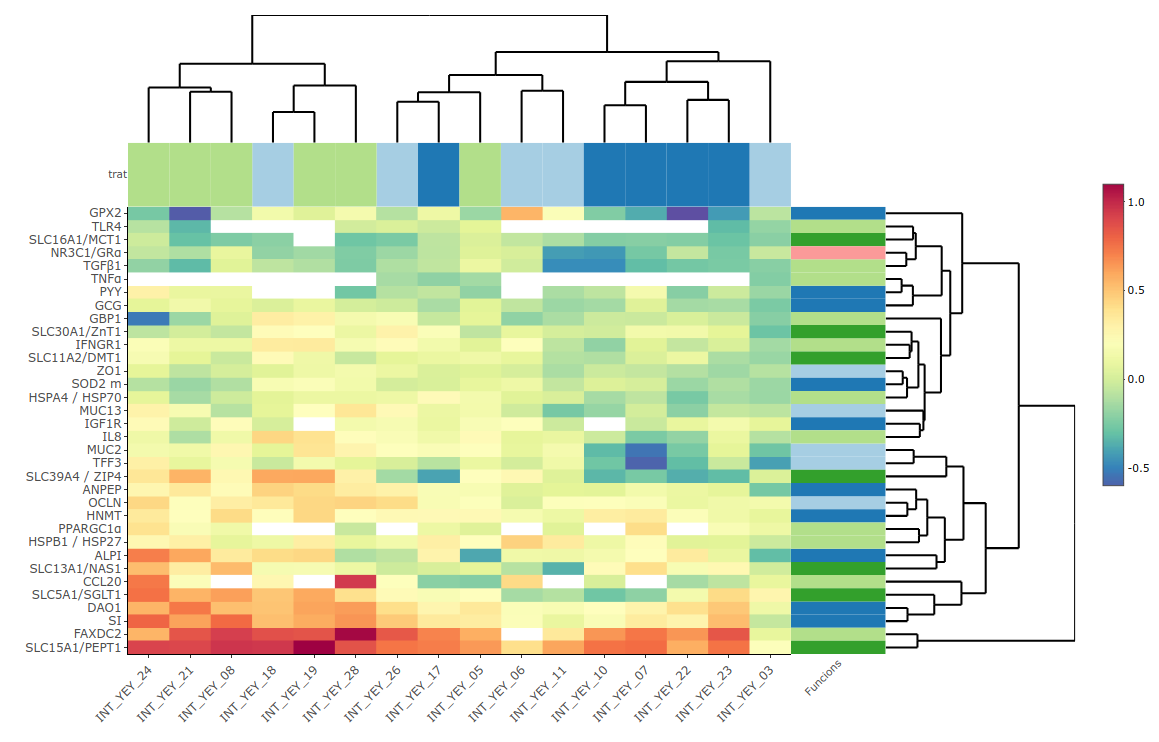
\includegraphics[scale=0.2]{heatmap.png}
\captionof{figure}{\texttt{Heatmap} generat a partir de 34 gens i 16 mostres. A les files trobem els gens i a les columnes les mostres. A més, es troben agrupats tant per gens com per mostres per mitjà d'un clúster jeràrquic. Per obtenir més informació, s'ha afegit variables fora de la matriu, concretament, a quin tractament correspon la mostra, i quina funció desenvolupa el gen.}
\end{center}

El mapa de calor també es pot combinar amb mètodes de \textit{clustering} que agrupen els gens i les mostres junts en funció de la similitud del seu patró d'expressió gènica. Això pot ser útil per identificar els gens que normalment s'expressen molt semblant i detectar patrons sota condicions o covariables establertes. El mètode implementat per la funció \texttt{heatmap}, utilitza l'anàlisi de clústers jeràrquics.
\\

En el cas dels mètodes jeràrquics les dades s'ordenen en nivells de manera que els nivells superiors contenen als inferiors. La jerarquia construïda permet obtenir també una partició de les dades en grups. S'utilitza la matriu de distàncies o similituds entre els elements de la matriu original de les dades.
\\

Els algoritmes \textit{jeràrquics} poden ser de dos tipus: De divisió i d'Aglomeració.
\\

L'\textit{algoritme de divisió} assumeix que en un primer pas totes les dades conformen un sol conglomerat. Aquest clúster es va dividint successivament en conglomerats més petits d'acord a algun criteri seleccionat prèviament. El resultat d'aquest procediment es representa pel dendrograma.
\\

L'\textit{algoritme d'aglomeració} assumeix que cada observació inicialment és un conglomerat i en cada pas s'associen els conglomerats més similars fins a arribar a un sol clúster.
\\

La implementació \texttt{hclust} (\textit{hierarchical cluster analysis}) de \texttt{R} utilitza el mètode  \textit{Mètode de Ward} que calcula i actualitza a cada pas la dissimilaritat entre clústers, aquest mètode és d'aglomeració.
\\
\clearpage
\noindent\textbf{Mètode de Ward}
\\
%http://www.ugr.es/~gallardo/pdf/cluster-3.pdf

\noindent Ward va proposar que la pèrdua d'informació que es produeix en integrar els diferents individus en clústers pot mesurar-se a través de la suma total dels quadrats de les desviacions entre cada punt (individu) i la mitjana del clúster en el qual s'integra. Perquè el procés de clusterització resulti òptim, en el sentit que els grups formats no distorsionin les dades originals, proposava la següent estratègia:
\\

A cada pas de l'anàlisi, es considera la possibilitat de la unió de cada parell de grups i optar per la fusió d'aquells dos grups que menys incrementin la suma dels quadrats de les desviacions en unir-se.
\\

Definim:
\begin{itemize}
\item $x_{ij}^k$ com el valor de la j-èssima variables sobre l'i-èssim individu del k-èssim clúster, suposant que aquest clúster té $n_k$ individus.
\item $m^k$ com el centroide del clúster $k$, amb components $m_{j}^k$
\item $E_k$ com la suma de quadrats dels errors del clúster $k$, és a dir, la distancia euclídea al quadrat entre cada individu del cluster $k$ al seu centroide:
\begin{equation*}
E_k = \sum_{i=1}^{n_k}\sum_{j=1}^{n}(x_{ij}^k - m_{j}^k)^2
\end{equation*}
\item $E$ com la suma de quadrats dels errors per a tots els clústers, és a dir, si suposem $h$ clústers:
\begin{equation*}
E = \sum_{k=1}^{h} E_k
\end{equation*}
\end{itemize}
El procés comen\c{c}a amb $m$ clústers, cada clúster només té un sol individu, per tant, cada individu coincideix amb el centre del clúster i en aquest primer pas $E_k=0$, per a cada clúster i això fa que $E=0$. L'objectiu del mètode de Ward és trobar en cada etapa aquells dos clústers els quals la seva unió proporcioni el menor increment en la suma total d'errors $E$. Suposem que els clústers $C_p$ i $C_q$ s'uneixen resultant un nou clúster $C_t$, llavors definim l'increment de $E$ com,
\begin{equation*}
\bigtriangleup E_{pq} = E_t - E_p - E_q
\end{equation*}
el procés es repeteix fins a l'obtenció del dendrograma i l'agrupació dels individus en els diferents clústers. Un exemple aclaridor d'aquest procés iteratiu, amb dades reals, es pot trobar a l'annex \ref{annex:a}.
\\

\textbf{Observació.} El mètode de Ward és un dels més utilitzats en la pràctica; posseeix gairebé tots els avantatges del mètode de la mitjana i sol ser més discriminant en la determinació dels nivells d'agrupació. Una investigació duta a terme per Kuiper i Fisher va provar que aquest mètode era capa\c{c} d'encertar millor amb la classificació òptima que altres mètodes.
\subsubsection{Biplot}
%http://www.knowledgeviz.com/pdf/UKC2009.pdf
L'anàlisi de components principals és una de les diferents maneres per analitzar l'estructura d'una matriu de correlacions donada. En aquest apartat parlarem del biplot, un tipus de gràfic exploratori on s'analitzen les correlacions entre les variables.
\\

Les components principals
\\

El biplot aproxima la distribució d'una mostra multivariant en un espai de dimensió reduïda, normalment de dues dimensions, i superposa sobre la mateixa gràfica les representacions de les variables sobre les quals es mesura la mostra. Un biplot permet mostrar gràficament la informació de les files (individus, casos, etc, ...) i les columnes (variables) d'una matriu de dades multivariants. El prefix bi es refereix a aquest fet i no al fet que el gràfic es fa normalment en dues dimensions.
\\

\noindent Podem veure un exemple a la següent figura:
\begin{center}
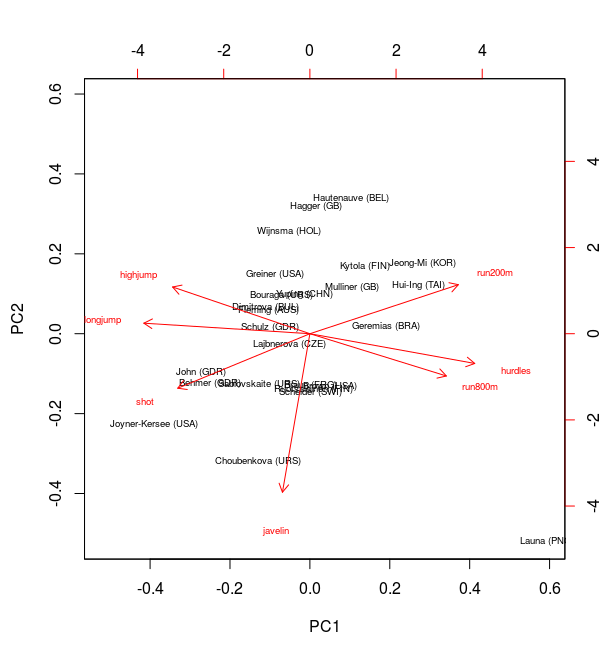
\includegraphics[scale=0.55]{biplot.png}
\captionof{figure}{ Biplot de les dues primeres components (dades escalades). Aquest és un exemple que es pot trobar al llibre \textit{A Handbook of Statistical Analyses Using R. Brian S. Everitt and Torsten Hothorn}. Les dades corresponen als resultats de 25 competidors en 7 proves esportives.}
\end{center}
El gràfic esta format per:
\begin{itemize}
\item La puntuació per a cada individu (atletes) en les dues primeres components principals. (Eix esquerra i eix inferior)
\item Els \textit{loadings} per a cada variable (esdeveniments esportius) en les dues primeres components principals. (Eix dreta i eix superior)
\end{itemize}
En general el biplot serà més representatiu de l'estructura dels casos i les variables si les dues components escollides expliquen una quantitat suficient de la variància.


%%% RESULTS
\clearpage
\section{Cas d'estudi}
El cas d'estudi consisteix en un disseny experimental fet amb porcins que han sigut alimentats amb diferents fonts de proteïnes (diverses combinacions de productes de soja, plasma animal i mucosa) a principis del deslletament. L'objectiu principal del estudi és avaluar la salut intestinal del porc poc després d'administrar les diferents dietes. A més, és vol veure si els tractaments tenen un efecte en el creixement del porc, i per tant, en la productivitat de l'empresa.
\subsection{Descripció de l'estudi}
L'estudi es defineix breument en els següents punts\\

\noindent\textbf{Objectiu de l'estudi}
\begin{itemize}
  \item Analitzar i comparar els diferents tractaments i com afecten a l'expressió dels gens.
  \item Trobar relacions entre la funcionalitat del gen i la seva expressió sota diferents tractaments.
\end{itemize}
\noindent\textbf{Disseny de l'estudi}\\
Estudi experimental amb una mostra total de 46 casos.
\noindent\textbf{Tractaments}
\begin{itemize}
  \item \textbf{T1}: Inclusió d'aliments de soja a la dieta.
  \item \textbf{T2}: Inclusió de plasma animal a la dieta.
  \item \textbf{T3}: Inclusió de $33\%$ de plasma animal i  $66\%$ de mucosa a la dieta.
  \item \textbf{T4}: Inclusió de $50\%$ de plasma animal i  $50\%$ de mucosa a la dieta.
\end{itemize}
\noindent\textbf{Variables explicatives}\\
La principal variable explicativa és:
\begin{itemize}
  \item Tractament
\end{itemize}
Les variables secundàries que també trobem a l'estudi:
\begin{enumerate}
  \item ID: nom del cas.
  \item Teixit: l'estudi es fa paral·lelament amb 2 tipus de teixits diferents, per tant, es farà un estudi amb cada teixit. (Dels 46 casos, queden 23 casos per teixit)
  \begin{itemize}
    \item Jejunum
    \item Ileum
  \end{itemize}
\end{enumerate}
\noindent\textbf{Variables genètiques}\\
Cada gen és una variable on es mesura l'abundancia de material genètic. Els gens han sigut escollits pels investigadors basant-se en les seves recerques i reben el nom de gens \textit{diana}. A l'annex \ref{annex:b} trobem una taula de tots els gens de l'estudi amb la seva funcionalitat dins de l'organisme.
\newpage
\noindent\textbf{Tractament de dades faltants}\\
El tractament dels NA’s és el següent:
\begin{enumerate}
\item S’eliminen aquelles files i columnes sense cap observació vàlida.
\item S’eliminen aquelles columnes (gens) que tinguin més del 50$\%$ de valors perduts en algun tractament.
\end{enumerate}
\noindent\textbf{Mètodes estadístics}\\
L'anàlisi estadístic ha sigut realitzat utilitzant \texttt{R} amb la versió 3.4.3.
\\

Per a tots els tests estadístics s'ha aplicat un nivell de significació del $5\%$ (P < 0.05). S'han realitzat correccions per multiplicitat de contrastos; \textit{Benjamini$\&$Hochberg} per l'ANOVA i \textit{Tukey} per les comparacions 2 a 2 entre tractaments.
\\

Tota la documentació, codi i \textit{outputs} han sigut emmagatzemats en un repositori públic a la plataforma \textit{GitHub}.\\
\noindent\textbf{Tractament de les dades}\\
Les dades han sigut validades abans de l'anàlisi, qualsevol inconsistencia en el format de les dades ha sigut eliminat o canviat. Més endavant s'expliquen quins criteris de l'estructura de la base de dades són els adequats perquè sigui funcional a l'aplicatiu.
\\

A més, hem aplicat una tranformació logarítmica als valors d'expressió gènica per a cada gen, amb l'objectiu de treballar amb una distribució normal i poder aplicar els mètodes estadístics descrits anteriorment.
\begin{center}
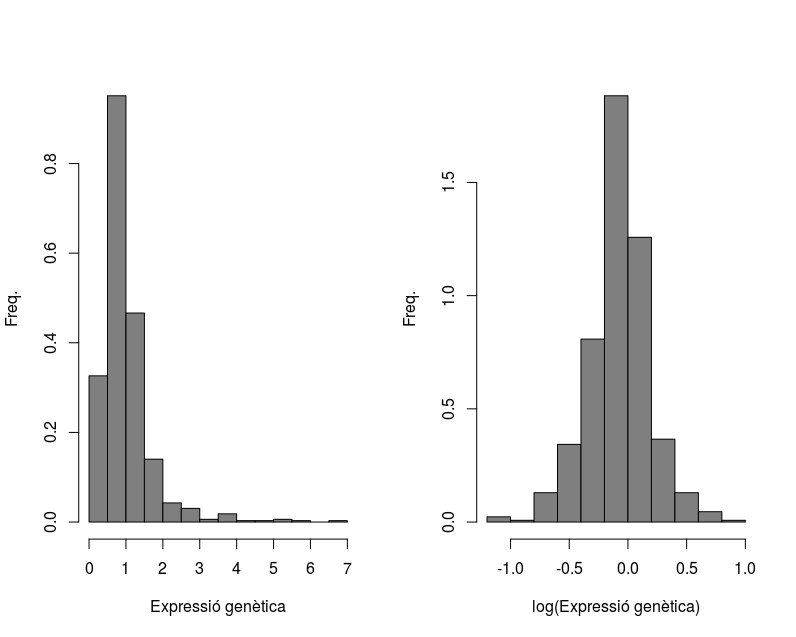
\includegraphics[scale=0.45]{logsdades.png}
\captionof{figure}{(1) El gràfic de l'esquerra mostra les dades sense cap tipus de transformació.(2) El gràfic de la dreta mostra les dades amb una transformació logarítmica.}
\end{center}
\clearpage
\subsection{Resultats}
Degut al disseny de l'estudi, s'analitzen paral·lelament 2 tipus de teixits, \textit{Ilenum} i \textit{Jejunum}. L'anàlisi que es duu a terme consta d'una primera part on s'examinen quins gens s'expressen diferencialment en cada teixit sota els 4 tractaments, i es determinen quins tractaments són diferents entre ells per a cada gen. Després hi ha una segona part més desciptiva on s'analitzen els patrons trobats en els mètodes visuals.
\subsubsection{Anàlisi de la variància (ANOVA)}
Amb l'objectiu de trobar quins gens s'expressen diferencialment sota els diferents tractaments s'ha aplicat l'anàlisi de la variancia per a cada teixit:
\begin{table}[ht]
\centering
\begin{tabular}{rlrrc}
    \toprule
{\textbf{Nom del gen}} & {\textbf{Funció del gen }} & {\textbf{Estadístic F}} & {\textbf{P-valor}} & {\textbf{P-valor (Benjamini$\&$Hochberg)}} \\
  \midrule
{\textcolor{gray}{TFF3}} & Barrier Function & 5.2927 & 0.0086 & $0.0603^{*}$ \\
  {\textcolor{gray}{OCLN}} & Barrier Function & 1.2861 & 0.3094 & 0.4572 \\
  {\textcolor{gray}{ZO1}} & Barrier Function & 0.9128 & 0.4544 & 0.5979 \\
  {\textcolor{gray}{MUC2}} & Barrier Function & 7.2461 & 0.0022 & $0.0272^{***}$ \\
  {\textcolor{gray}{MUC13}} & Barrier Function & 2.1769 & 0.1261 & 0.2425 \\
  {\textcolor{gray}{SI}} & Enzymed/Hormone & 3.1867 & 0.0488 & 0.1525 \\
  {\textcolor{gray}{DAO1}} & Enzymed/Hormone & 1.2813 & 0.3109 & 0.4572 \\
  {\textcolor{gray}{HNMT}} & Enzymed/Hormone & 0.5736 & 0.6396 & 0.6953 \\
  {\textcolor{gray}{ANPEP}} & Enzymed/Hormone & 1.9658 & 0.1553 & 0.2773 \\
  {\textcolor{gray}{GCG}} & Enzymed/Hormone & 1.1972 & 0.3390 & 0.4709 \\
  {\textcolor{gray}{IGF1R}} & Enzymed/Hormone &  &  &  \\
  {\textcolor{gray}{GPX2}} & Enzymed/Hormone & 10.5231 & 0.0003 & $0.0079^{***}$\\
  {\textcolor{gray}{SOD2m}} & Enzymed/Hormone & 3.3427 & 0.0424 & 0.1516 \\
  {\textcolor{gray}{ALPI}} & Enzymed/Hormone & 2.1929 & 0.1241 & 0.2425 \\
  {\textcolor{gray}{TNF$\alpha$}} & Inmune Response &  &  &  \\
  {\textcolor{gray}{TGF$\beta_1$}} & Inmune Response & 1.7353 & 0.1956 & 0.3260 \\
  {\textcolor{gray}{CCL20}} & Inmune Response &  &  &  \\
  {\textcolor{gray}{IFNGR1}} & Inmune Response & 4.5897 & 0.0148 & $0.0741^{*}$ \\
  {\textcolor{gray}{HSPB1.HSP27}} & Inmune Response & 0.8298 & 0.4947 & 0.6184 \\
  {\textcolor{gray}{HSPA4.HSP70}} & Inmune Response & 0.6819 & 0.5745 & 0.6529 \\
  {\textcolor{gray}{FAXDC2}} & Inmune Response &  &  &  \\
  {\textcolor{gray}{GBP1}} & Inmune Response & 0.6991 & 0.5647 & 0.6529 \\
  {\textcolor{gray}{IL8}} & Inmune Response & 5.1389 & 0.0096 & 0.0603 \\
  {\textcolor{gray}{SLC5A1.SGLT1}} & Nutrient Transport& 2.5431 & 0.0886 & 0.2013 \\
  {\textcolor{gray}{SLC16A1.MCT1}} & Nutrient Transport & 0.1985 & 0.8961 & 0.9334 \\
  {\textcolor{gray}{SLC15A1.PEPT1}} & Nutrient Transport &  &  &  \\
  {\textcolor{gray}{SLC13A1.NAS1}} & Nutrient Transport & 2.8547 & 0.0661 & 0.1652 \\
  {\textcolor{gray}{SLC11A2.DMT1}} & Nutrient Transport &  &  &  \\
  {\textcolor{gray}{SLC30A1.ZnT1}} & Nutrient Transport & 4.2445 & 0.0196 & $0.0818^{*}$ \\
  {\textcolor{gray}{SLC39A4.ZIP4}} & Nutrient Transport & 3.0217 & 0.0567 & 0.1575 \\
  {\textcolor{gray}{NR3C1.Gr$\alpha$}} & Stress & 0.0308 & 0.9925 & 0.9925 \\
   \bottomrule
\end{tabular}
\onecolumn
\caption{P-valors de l'ANOVA entre tractaments pel teixit \textbf{Ileum}. Els pvalors per sota de 0.05 queden marcats amb $^{***}$ i per sota de 0.1 amb $^{*}$.}
\end{table}

\noindent El nivell de significació és $\alpha$=0.05, però degut al conjunt de tests realitzats s'aplica una correcció (\textit{Benjamini $\&$ Hochberg}). Per tant, només s'haurien de considerar significatius del conjunt experimental aquells tests en els que el p-valor de \textit{Benjamini $\&$ Hochberg} estigui per sota de determinat llindar, en aquest cas hem fixat un nivell de significació del 5$\%$, encara que en aquests tipus d'experiments poden arrbiar al $10\%$. Observem que hi ha gens sense cap pvalor, això es degut a que després de fer el tractament de dades faltants (descrit a l'apartat anterior) encara hi ha NA's, per tant, l'anàlisi de la variància no contempla aquests gens.
%Jejunum
\onecolumn
\begin{table}[ht]
\centering
\begin{tabular}{rlrrc}
  \toprule
 {\textbf{Nom del gen}} & {\textbf{Funció del gen }} & {\textbf{Estadístic F}} & {\textbf{P-valor}} & {\textbf{P-valor (Benjamini$\&$Hochberg)}} \\
  \midrule
{\textcolor{gray}{TFF3}} & Barrier Function & 5.2048 & 0.0099 & $0.0635^{*}$  \\
  {\textcolor{gray}{OCLN}} & Barrier Function & 3.7353 & 0.0314 & $0.0919^{*}$  \\
  {\textcolor{gray}{ZO1}} & Barrier Function & 2.4161 & 0.1020 & 0.1962 \\
  {\textcolor{gray}{MUC2}} & Barrier Function & 5.0794 & 0.0108 & $0.0635^{*}$  \\
  {\textcolor{gray}{MUC13}} & Barrier Function & 2.1372 & 0.1332 & 0.2220 \\
  {\textcolor{gray}{SI}} & Enzymed/Hormone & 3.6748 & 0.0331 & $0.0919^{*}$  \\
  {\textcolor{gray}{DAO1}} & Enzymed/Hormone & 4.8678 & 0.0127 & $0.0635^{*}$  \\
  {\textcolor{gray}{HNMT}} & Enzymed/Hormone & 4.5122 & 0.0167 & $0.0697^{*}$  \\
  {\textcolor{gray}{ANPEP}} & Enzymed/Hormone & 2.3119 & 0.1126 & 0.2011 \\
  {\textcolor{gray}{GCG}} & Enzymed/Hormone & 6.6996 & 0.0035 & $0.0433^{***}$ \\
  {\textcolor{gray}{IGF1R}} & Enzymed/Hormone &  &  &  \\
  {\textcolor{gray}{PYY}} & Enzymed/Hormone &  &  &  \\
  {\textcolor{gray}{GPX2}} & Enzymed/Hormone &  &  &  \\
  {\textcolor{gray}{SOD2m}} & Enzymed/Hormone & 1.4329 & 0.2680 & 0.3526 \\
  {\textcolor{gray}{ALPI}} & Enzymed/Hormone & 1.0417 & 0.3994 & 0.4755 \\
  {\textcolor{gray}{TLR4}} & Inmune Response &  &  &  \\
  {\textcolor{gray}{TGF$\beta1$}} & Inmune Response & 1.7069 & 0.2034 & 0.3178 \\
  {\textcolor{gray}{CCL20}} & Inmune Response &  &  &  \\
  {\textcolor{gray}{IFNGR1}} & Inmune Response & 1.5036 & 0.2495 & 0.3526 \\
  {\textcolor{gray}{HSPB1.HSP27}} & Inmune Response & 0.3366 & 0.7991 & 0.8324 \\
  {\textcolor{gray}{HSPA4.HSP70}} & Inmune Response & 0.8326 & 0.4943 & 0.5617 \\
  {\textcolor{gray}{FAXDC2}} & Inmune Response &  &  &  \\
  {\textcolor{gray}{GBP1}} & Inmune Response & 0.0084 & 0.9989 & 0.9989 \\
  {\textcolor{gray}{IL8}} & Inmune Response & 2.5729 & 0.0881 & 0.1835 \\
  {\textcolor{gray}{SLC5A1.SGLT1}} & Nutrient Transport & 4.1519 & 0.0223 & $0.0796^{*}$  \\
  {\textcolor{gray}{SLC16A1.MCT1}} & Nutrient Transport &  &  &  \\
  {\textcolor{gray}{SLC15A1.PEPT1}} & Nutrient Transport & 2.9677 & 0.0613 & 0.1394 \\
  {\textcolor{gray}{SLC13A1.NAS1}} & Nutrient Transport & 3.5486 & 0.0368 & $0.0921^{*}$  \\
  {\textcolor{gray}{SLC11A2.DMT1}} & Nutrient Transport & 1.3570 & 0.2895 & 0.3618 \\
  {\textcolor{gray}{SLC30A1.ZnT1}} & Nutrient Transport & 0.4630 & 0.7118 & 0.7737 \\
  {\textcolor{gray}{SLC39A4.ZIP4}} & Nutrient Transport & 19.3772 & 0.0000 & $0.0003^{***}$ \\
  {\textcolor{gray}{NR3C1.Gr$\alpha$}} & Stress & 1.4606 & 0.2606 & 0.3526 \\
   \bottomrule
\end{tabular}
\caption{P-valors de l'ANOVA entre tractaments pel teixit \textbf{Jejunum}. Els pvalors per sota de 0.05 queden marcats amb $^{***}$ i per sota de 0.1 amb $^{*}$.}
\end{table}
\clearpage
\onecolumn
\subsubsection{Comparacions múltiples 2 a 2}
\begin{table}[ht]
\centering
\scalebox{1}{
\begin{tabular}{rrrrrrr}
  \toprule
 & {\textbf{2-1}} & {\textbf{3-1}} & {\textbf{4-1}} & {\textbf{3-2}} & {\textbf{4-2}} & {\textbf{4-3}} \\
  \midrule
{\textcolor{gray}{TFF3}} & 0.3188 & 0.3478 & 0.0044 & 0.9990 & 0.1862 & 0.1238 \\
  {\textcolor{gray}{MUC2}} & 0.0399 & 0.6594 & 0.0023 & 0.2903 & 0.5807 & 0.0243 \\
  {\textcolor{gray}{GPX2}} & 0.0028 & 0.8767 & 0.0632 & 0.0006 & 0.5016 & 0.0147 \\
  {\textcolor{gray}{IFNGR1}} & 0.6521 & 0.0625 & 0.0160 & 0.5062 & 0.1856 & 0.8559 \\
  {\textcolor{gray}{IL8}} & 0.0203 & 0.7625 & 0.0329 & 0.1273 & 0.9959 & 0.1907 \\
  {\textcolor{gray}{SLC30A1.ZnT1}} & 0.8488 & 0.0984 & 0.3940 & 0.0249 & 0.1293 & 0.8790 \\
   \bottomrule
\end{tabular}
}
\caption{Dels gens significatius per al teixit \textbf{Ilenum}, s'apliquen comparacions per multiplicitat de contrastos Gene-Tractament}
\end{table}
\begin{table}[ht]
\centering
\scalebox{1}{
\begin{tabular}{rrrrrrr}
  \toprule
 & {\textbf{2-1}} & {\textbf{3-1}} & {\textbf{4-1}} & {\textbf{3-2}} & {\textbf{4-2}} & {\textbf{4-3}} \\
  \midrule
{\textcolor{gray}{TFF3}} & 0.3103 & 0.7306 & 0.2612 & 0.0512 & 0.0074 & 0.8416 \\
  {\textcolor{gray}{OCLN}} & 0.7919 & 0.2620 & 0.3580 & 0.0510 & 0.0713 & 0.9903 \\
  {\textcolor{gray}{MUC2}} & 0.2886 & 0.6525 & 0.3436 & 0.0357 & 0.0098 & 0.9583 \\
  {\textcolor{gray}{SI}} & 0.8958 & 0.4620 & 0.0283 & 0.8557 & 0.1154 & 0.4220 \\
  {\textcolor{gray}{DAO1}} & 0.9388 & 0.0422 & 0.0368 & 0.1245 & 0.1152 & 0.9999 \\
  {\textcolor{gray}{HNMT}} & 0.4370 & 0.0211 & 0.0357 & 0.3378 & 0.5138 & 0.9766 \\
  {\textcolor{gray}{GCG}} & 0.9985 & 0.0896 & 0.0142 & 0.0662 & 0.0100 & 0.8457 \\
  {\textcolor{gray}{SLC5A1.SGLT1}} & 0.9227 & 0.2469 & 0.1394 & 0.0842 & 0.0410 & 0.9937 \\
  {\textcolor{gray}{SLC13A1.NAS1}} & 0.1100 & 0.2227 & 0.0286 & 0.9754 & 0.9335 & 0.7387 \\
  {\textcolor{gray}{SLC39A4.ZIP4}} & 0.0015 & 0.3812 & 0.1450 & 0.0001 & 0.0000 & 0.9453 \\
   \bottomrule
\end{tabular}
}
\caption{Dels gens significatius per al teixit \textbf{Jejunum}, s'apliquen comparacions per multiplicitat de contrastos Gene-Tractament}
\end{table}
\subsubsection{Mètodes visuals}
\subsection{Conclusions}
%%Shiny
\section{TL3P: Aplicatiu Web amb el paquet \texttt{Shiny} de R}
\subsection{Introducció a Shiny}
\subsubsection{Estructura de l'aplicatiu}
\subsubsection{Gestió i control de versions}
\subsection{Funcionalitats de l'aplicació}
\subsection{Desenvolupament i futures versions}
%Bibliografia
\begin{thebibliography}{9}
\bibitem{caca8}
Mark D. Robinson, Davis J. McCarthy, Gordon K. Smyth; edgeR: a Bioconductor package for differential expression analysis of digital gene expression data, Bioinformatics, Volume 26, Issue 1, 1 January 2010, Pages 139–140,
\\\texttt{https://doi.org/10.1093/bioinformatics/btp616}

\bibitem{caca7}
K. R. GABRIEL; The biplot graphic display of matrices with application to principal component analysis, Biometrika, Volume 58, Issue 3, 1 December 1971, Pages 453–467, \\\texttt{https://doi.org/10.1093/biomet/58.3.453}

\bibitem{caca2}
Ramón Tamarit Agusti. Análisis de cluster no supervisados. Aplicaciones en
la búsqueda y visualización de perfiles de expresión
en datos de microarrays.
\\\texttt{http://mural.uv.es/rata3/PECSspace.html}

\bibitem{pca}
Dong Hyun Jeong, Caroline Ziemkiewicz, William Ribarsky and Remco Chang: Understanding Principal Component Analysis Using a Visual Analytics Tool,
\\\texttt{http://www.knowledgeviz.com/pdf/UKC2009.pdf}

\bibitem{caca1}
Universidad de Granada: Comparaciones múltiples.
\\\texttt{http://wpd.ugr.es/$\sim$bioestad/guia-spss/practica7}

\bibitem{caca}
Universidad de Granada: Métodos de análisis multivariante. Análisis clúster.
\\\texttt{http://wpd.ugr.es/$\sim$bioestad/guia-spss/}

\bibitem{cl}
Universidad de Granada: Métodos Jerárquicos de Análisis Cluster.
\\\texttt{http://www.ugr.es/$\sim$gallardo/pdf/cluster-3.pdf}

\bibitem{caca5}
\textit{NCBI, National Center of Biotechnology Information.}
\\\texttt{https://www.ncbi.nlm.nih.gov/}. USA

\bibitem{caca6}
\textit{PubMed. US National Library of Medicine.}
\\\texttt{https://www.ncbi.nlm.nih.gov/pubmed/}. USA

\end{thebibliography}
%%Appendix
\clearpage
\appendix
\onecolumn
\section{Mètode de Ward: Exemple del mètode amb gens}
\label{annex:a}
Observem com funciona aquest mètode en el cas de tenir 3 gens on es mesura l'expressió gènica per a 3 mostres. Les dades són les següents:
\begin{table}[ht]
\centering
\begin{tabular}{rrrr}
\hline
& $X_{1}$ & $X_2$ & $X_3$ \\
\hline
$Gen_1$ & 1.02 & 0.21 & 6.29 \\
$Gen_2$ & 10.06 & 8.19 & 7.29 \\
$Gen_3$ & 10.11 & 14.63 & 7.62 \\
\hline
\end{tabular}
\caption{Expressió gènica de cada gen $Gen_i$ per a cada mostra $X_j$.}
\end{table}
\\
Recordem que per utilitzar aquest mètode necessitem la matriu de distàncies euclidianes. La distància euclidiana entre dos punts ${\displaystyle \,P=(p_{1},p_{2},\dots p_{n})}$ i $ {\displaystyle \,Q=(q_{1},q_{2},\dots q_{n})}$ es defineix com:
\begin{equation*}
{\displaystyle d_{E}(P,Q)={\sqrt {(p_{1}-q_{1})^{2}+(p_{2}-q_{2})^{2}+\cdots +(p_{n}-q_{n})^{2}}}}
\end{equation*}
Per tant, obtenim aquesta matriu de distàncies:
\begin{table}[ht]
\centering
\begin{tabular}{rrrr}
\hline
& $Gen_1$ & $Gen_2$ & $Gen_3$ \\
\hline
$Gen_1$ & 0 & 12.10 & 17.10 \\
$Gen_2$ & 12.10 & 0 & 6.45 \\
$Gen_3$ & 17.10 & 6.45 & 0 \\
\hline
\end{tabular}
\caption{Matriu de distàncies. La distància utilitzada és l'euclidiana.}
\end{table}
\\
En aquest cas, com tenim només 3 gens, tenim un total de 3 combinacions possibles de 2 elements. Per tant, calcularem $\bigtriangleup E$ per a cada combinació i escollirem el més petit com el millor clúster.
\\

\begin{table}[ht]
\onecolumn
\centering
\begin{tabularx}{\linewidth}{llllll}
\hline
& $Particions$ & $Centroides$ & $E_k$ & $E$ & $\bigtriangleup E$ \\
\hline
& $(Gen_1,Gen_2),Gen_3$ & $C_{Gen_1,Gen_2} = (5.54,4.19,6.78) $ & $E_{Gen_1,Gen_2}=72.92$
$E_{Gen_3}=0$ & $72.92$ & $72.92$ \\
& $(Gen_1,Gen_3),Gen_2$ & $C_{Gen_1,Gen_2} = (7.06,7.67,7.06) $ & $E_{Gen_1,Gen_3}=112.42$
$E_{Gen_2}=0$ & $112.42$ & $112.42$ \\
& $(Gen_2,Gen_3),Gen_1$ & $C_{Gen_1,Gen_2} = (10.08,11.41,7.45)$ & $E_{Gen_2,Gen_3}=20.79$
$E_{Gen_1}=0$ & $20.79$ & $20.79$ \\
\hline
\end{tabularx}
\caption{Taula resum dels càlculs proposats per obtenir l'increment de la suma de quadrats residuals. Les particions són possibles combinacions de 2 gens en un total de 3.}
\end{table}

\noindent Podem observar que segons el criteri de Ward, escolliríem unificar el $Gen_2$ i el $Gen_3$ en un mateix clúster. Si fem el mateix però automàticament amb la funció \texttt{hclust}, obtenim el següent dendrograma:
\begin{center}
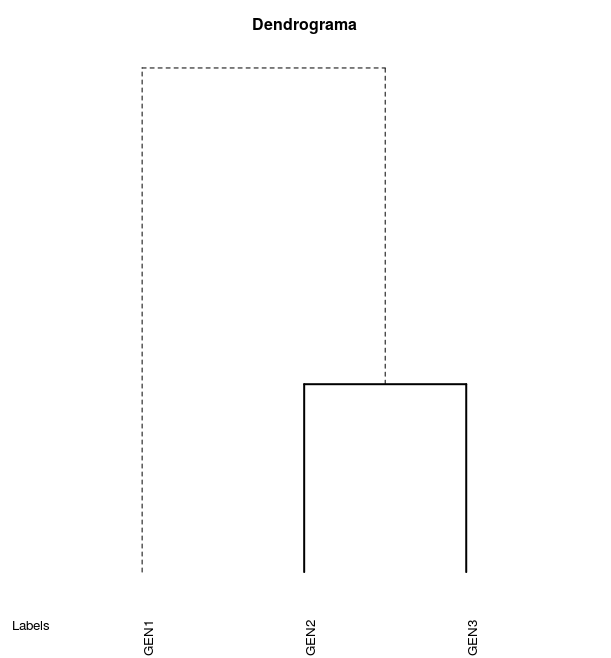
\includegraphics[scale=0.4]{dendrograma.png}
\captionof{figure}{Dendrograma obtingut amb la funció \texttt{hclust}. Si apliquem directament la funció \texttt{hclust}, que utilitza el mètode de Ward, obtenim 2 clústers. El primer clúster amb el $Gen_1$ i un segon clúster amb el $Gen_2$ i el $Gen_3$. Trobem els mateixos clústers amb el procediment manual que hem calculat anteriorment.}
\end{center}
\section{Gens diana utilitzats a l'estudi}
\label{annex:b}
\begin{center}
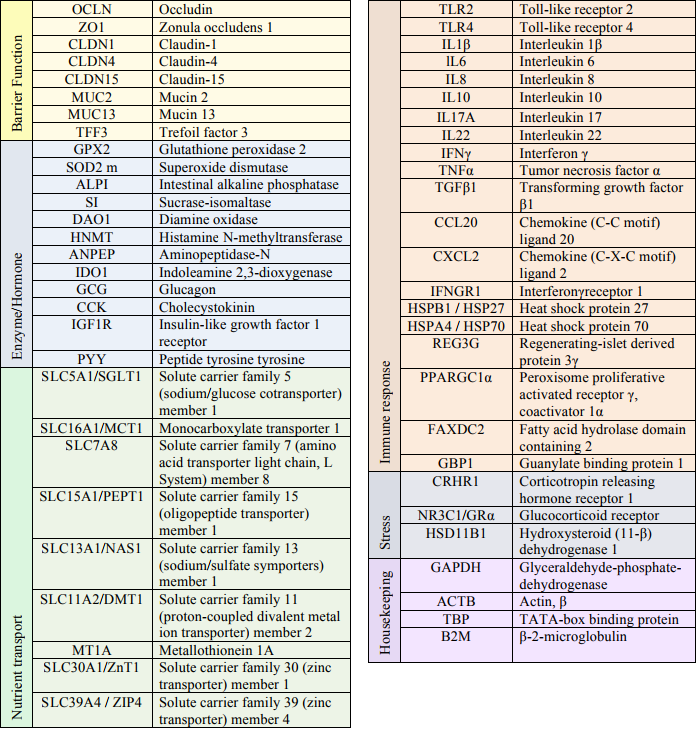
\includegraphics[scale=0.7]{genes.png}
\captionof{figure}{Gens \textit{diana} i la seva funció dins de l'organisme.}
\end{center}
\end{document}
